%
%  $Author: awl8049 $
%  $Date: 2008/06/25 02:17:17 $
%  $Revision: 1.8 $
%
%\documentclass[times, 10pt,twocolumn]{article} 
\documentclass[times, 10pt,onecolumn]{article} 
\usepackage{setspace}
\usepackage{latex8}
\usepackage{graphicx}
\usepackage{authblk}
\usepackage{amsmath}
\usepackage{amsthm}
%\usepackage{pdfsync}
\pagestyle{empty}
\begin{document}
\title{Efficient Systemwide Power Modeling for Server Environments}
\author[*]{}
% \author[*]{Adam Lewis} 
% \author[*]{Soumik Ghosh} 
% \author[*]{N.-F. Tzeng}
% \affil[*]{Center for Advanced Computer Studies\\ 
% University of Louisiana at Lafayette\\ 
% Lafayette, LA 70504, USA\\ 
% \{awlewis,sxg5317,tzeng\}@cacs.louisiana.edu
% }
\maketitle
\newtheorem{defn}{Definition}
\newtheorem{thm}{Theorem}
\thispagestyle{empty}
\doublespacing

\begin{abstract}
  The upwardly spiraling operating costs of the infrastructure for
  large-scale computing demand better power management in server
  environments.  High economic incentives exist to operate the data
  center at its full power capacity as much as possible.  This is
  difficult to achieve in practice, however, as the data center usually
  has over-provision in its power capacity for handling the worst case
  situations. As a result, there is considerable unused capacity
  available for other purposes.

  Thus, it is critical to quantitatively understand power consumption
  trends at the system level to maximize the use of deployed power
  capacity in the data center. Current approaches to power modeling
  focus either on the large scale issues in data center design or on a
  particular system component such as the processor or disk drive.

  This paper introduces an integrated system power model that provides
  fast and accurate prediction of power consumption in server
  installations.  The model is based on operating system metrics and
  performance counters to predict power consumption without the
  requirement of calibration.  The model is experimentally validated
  using statistical methods under a variety of actual application
  workloads.
\end{abstract}

\section{Introduction}
\label{sec:Introduction}
The heart of the infrastructure of today's information economy is the
data centers containing the servers that support most Internet services.
Such centers host hundreds or even thousands of servers running
off-the-shelf hardware.  The power demands of these installations force
firms to install complex and costly cooling solutions to efficiently
move the heat away from servers so as to avoid reliability problems.

Providing proper cooling has become more difficult as the density of the
off-the-shelf hardware has increased with tighter packaging, decreasing
form factors, and increasing performance demands.  The introduction of
multi-core processors combined together in clusters of traditional and
blade servers has greatly increased the power demands of servers.

Server systems, per \cite{Bianchini2004}, have characteristics that make
traditional power management techniques undesirable:
\begin{itemize}
\item server hardware is typically provisioned for peak load, and thus
  exhibit high performance and power consumption;
\item high availability and high bandwidth is typically provided by widespread
  replication of resources such as clusters of machine and disk arrays;
\item server power supplies must be able to store capacity to deal with sudden
  spikes in load and as result exhibit high power losses.
\end{itemize}

Application servers pose an especially interesting power management problem due
to intensive CPU and memory requirements combined with maintaining soft state
that is not typically replicated.   Intensive CPU and memory use means that
traditional power management mechanisms may impose too excessive demands upon
performance while non-replicated state forces state migration in order to turn
application servers on and off.

Barroso \textit{et.al.} \cite{Barroso2007} introduce the idea of
``energy-proportional machine'': a computer that exhibits a wide
dynamic power range and is capable of operating at lower power modes.
Prior work done for mobile devices can be of benefit to server systems
but that work needs to be enhanced for server devices that spend most of
their time at moderate utiliziation with less than peak efficiency.

Extensive study of the power profiles of the Intel Pentium architecture
has occured at the workstation \cite{Isci2003a} \cite{Isci2003b}
\cite{Isci2006} and server \cite{Bircher2004} \cite{Bircher2007}
\cite{Lee2005}.  However, very little consideration has been given to
the power profiles of servers constuctued using the {NUMA}-based
architecture used on processors such as the AMD64 family of processors
\cite{AMD2007}.  In contrast
to processors using a traditional frontside bus to communicate with the
outside world, these processors use a HyperTransport (HT) based bus
\cite{HT2007} to communicate between processors and the outside world.

There are two keys to creating an ``energy-proportional server'': an
accurate power model and a power predictor that implements that model.
This work contributes the following that can be used with NUMA-based processor
to create an energy-proportional server:
\begin{itemize}
\item A statistical full-system model of the power consumption of
  a NUMA-based processor that uses sensor data collected with through the
  out-of-band management controller with performance counter information
  collected from the system processor.
\item A detailed experimental study of the model.
\item Power prediction software that works in conjunction with the
  operating system kernel to predict when the system needs to scale back
  voltage or frequency to reduce the power consumption on the individual server.
\end{itemize}

The remainder of this paper is structured as follows: section
\ref{sec:related} describes related work.  Section \ref{sec:model}
describes the structure of the model.  Section \ref{sec:experiment}
shows our experimental results.  Section \ref{sec:conclusions} offers
our conclusions.

\section{Related Work}
\label{sec:related}
The techniques used for mobile and desktop computers have been applied
with some sucess to managing the power consumption of microprocessors
used in server hardware.  A common approach is the application of
dynamic voltage scaling: reducing the voltage (and as a result, the
frequency) of the processor at the cost of slower program
execution. Other approaches such as the approach taken by Intel with the
Pentium 4 processor have utilized a stop-go approach: activate and
deactivate the processor as demanded by workload.  These approaches have
mostly been applied most often to battery-powered devices.  They adjust
components to lowest power-mode that does not over-compromise
performance.  These transitions occur based on analysis of workload or
higher-level operation.

An examination of server activity patterns \cite{Fan2007}\cite{Barroso2007}
shows that servers are rarely completely idle and seldom operate near their
maximum utilization.   Analysis of server traces indicate that this behavior
is a result of two factors: the need to provision servers for the worst case
and the fact that application factors prevent extensive idle time on servers.
For Internet workloads, quality of service requirements mean that sufficient
slack be provided for the server to deal with potential server faults.
Furthermore, servers rarely become completely idle.   Data is distributed
across all servers in the server farm meaning that the server cannot become
completely idle if the data must always be available.  

Extensive study has been done on limiting the power consumption of
storage devices \cite{Pinheiro2004} and main memory \cite{Diniz2007}.
These approaches focus on these devices as the greatest energy consumers
in the system after the processor.  However, these approaches optimize
only one part of the system.  This is problematic because the system
compoenents interact with other and focusing on just one piece of the
energy consumption model may not be optimal from the standpoint of the
complete system.  An effective power model must take in account the
impact of these interactions.

Effective power modeling requires the use of a full-system approach.
How this is done falls into two schools of thought: modeling the power
at the simulation level, or attempting to correlating power consumption
to system-level metrics (at either the user or kernel level of the
operating system).

Power modeling through simulation using systems such as Wattach
\cite{Brooks2000} and HotSpot
\cite{Skadron2004} can provide detailed analysis and breakdown across
components in a system.    Simulation techniques have both speed and
scale issues.  Simulators are slow compared to the real hardware and do
not scale very well to long-running applications and large
data-sets. They are not an effective solution when real-time prediction
and dynamic optimization is required.

Another approach is to coorelate power consumption to phases of
application execution using system-level metrics.  The approaches used
to define this mapping fall into two categories: determining the
application phase using from either the control flow of the application
\cite{Hu2005} \cite{Iyer2001} \cite{Sherwood2003} or from performance
counter signatures of the executed instructions or operating system
metrics \cite{Bellosa2003} \cite{Isci2003a} \cite{Isci2003b}
\cite{Contreras2005} \cite{Economou2006}.  Attempts have been made to
reconcile these approaches by attempting to map programs phases to
events \cite{Isci2006}.

Models based on performance counter events and/or operating system
metrics are based on linear regression techniques where the authors
attempt to map a linear model of the collected metrics to the energy
consumed during the execution of a program 
 \cite{Isci2003c} \cite{Contreras2005}\cite{Bircher2007}.  

\section{The Model}
\label{sec:model}
Our model for computing the energy consumption of a single server blade
is based on computing the energy consumption of the 
computational and electromechanical elements that make up a server
blade. The model aims to develop a relationship between the
computational workload of the server and the various components of the
server to better understand the energy-dissipation dynamics within a
single server blade. This relationship between the computational
workload and energy-dissipation in various server components (processor,
HDD, main memory, fans, peripherals, etc.) can be used to accomplish the
following tasks:

\begin{itemize}
\item Computational load based dynamic monitoring of per blade energy
consumption
\item Energy-aware resource provisioning for the node and also for the
cluster
\item Energy-budget-aware computation and resource provisioning for
virtual machines running on a single node
\item Energy-aware load balancing for a scheduler
\end{itemize}
 \begin{figure}[ht]
   \begin{minipage}[b]{0.5\linewidth}
     \centering
     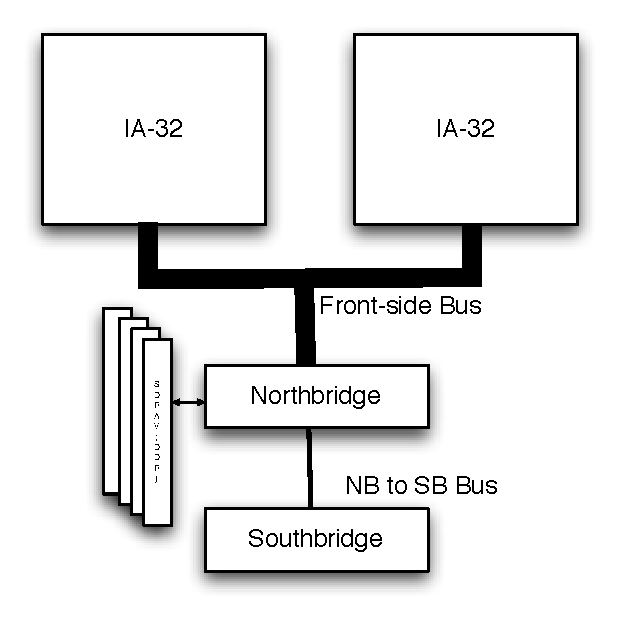
\includegraphics[scale=0.50]{intelarch.pdf}
     \caption{Intel Core Server Architecture}
     \label{fig:intarch}
   \end{minipage}
   \hspace{0.5cm}
   \begin{minipage}[b]{0.5\linewidth}
     \centering
     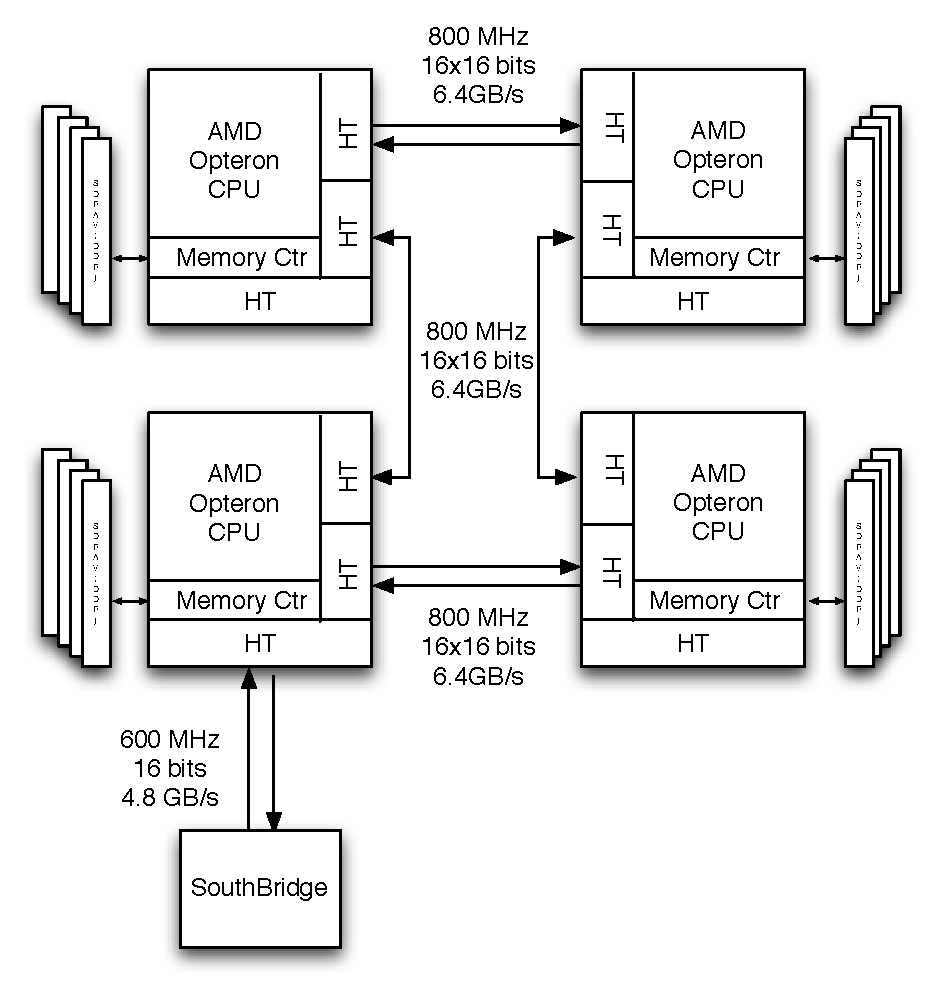
\includegraphics[scale=0.50]{amdhtarch.pdf}
     \caption{AMD Opteron Server Architecture}
     \label{fig:optarch}
   \end{minipage}
 \end{figure}

In order to a get a true measure of the computational load on the
system, our method looks to snoop on completed bus transactions per unit
time in a system and measure the relative change in energy consumption
(as indicated by change in temperature) as computation tasks as
completed.   Use of this performance counter metric as compared to other
metrics fits well with the architecture of microprocessors used in
NUMA-based processors in multicore environments.   

Consider how the Intel Pentium and AMD Operton
processor architectures shown in Figure \ref{fig:intarch} and
\ref{fig:optarch}.  The Pentium architecture (and its successors) is based
upon the idea of a Front-Side-Bus (FSB) which connects individual cores to the
Northbridge chip.  This chip provides the interface between the cores and
memory.  A coherent bus protocol is used to ensure consistency in memory
access between the cores.  For this architecture, the FSB becomes a
performance bottleneck as processor and cores have to moderate themselves to
the slower speed of the bus.  

Contrast this with the NUMA-based architecture used by the AMD Opteron (Figure
\ref{fig:amdarch}).  In this case, the Northbridge functionality is combined
onto the same processor die as each core and each core is responsible for
local access to the memory connected to that Northbridge.    Cores on a single
die are connected via a crossbar to the Hypertransport bus between
processors.  Again a coherent bus protocol is used to ensure memory
consistency between cores and processors.   In addition, the master processor
in the system is connected via a second Hypertransport bus to the Southbridge
device that manages connections to the outside world.

We see that computation will result in bus traffic along
either the HT buses that connect the processors or the HT bus that
connects the master processor to pepherial bridge processor.  The
infomation passed along the bus between the processors, when combined
with performance counter information about L2 cache misses, can be used
as an estimator of the energy consumed by movement of data to and from
memory.  The amount of data flowing through the bus between the
root-node processor and the Southbridge provides us with an estimator of
the energy consumption required to communicate with the outside world.

In a processor, during computation, as the processor executes
its sequence of instructions and operates on the given data, energy is
consumed due to the amount of switching activity taking place within a
processor. In fact from an IC design standpoint, this energy consumption
per unit time is broadly given by :

\begin{equation}
\label{eq:power_proc}
P_{processor}=  \alpha*C*V_{dd}^2*f + I_{static}*V_{dd} + V_{dd}*I_{leakage}
\end{equation}

where $\alpha$ is the switching activity in the first term which is the
\emph{dynamic power consumption}, $V_{dd}$ is the supply voltage, $C$ is
the total associated capacitance, $I_{static}$ is the static current
flowing when there is no activity (switching), and $I_{leakage}$ is the
leakage current due to low threshold voltages in the processor. In
general, the attempt is to reduce the first term, as it is the dominant
energy consuming term in the equation. Besides reducing the operating
voltage, clock frequency and total chip capacitance, a lot of
architectural effort goes into reducing $\alpha$ which is known as the
\emph{activity factor}, or in other words, the switching probability.

The first task in estimating the power consumption of a digital system
is to identify the typical application programs that will be executed on
the system. A non-trivial application program consumes millions of
machine cycles, making it hard to get power estimate for a particular
application. In \cite{Sato1995} the power cost of a CPU module is
characterized by estimating the average capacitance that would switch
when the CPU module is activated. In \cite{Su1994} , the switching
activities on buses (address, instruction, data) are used to estimate
the power consumption of the microprocessor. In \cite{Tiwari1994},
based on actual current measurements of some processors, the following
instruction-level power mode is proposed:

\begin{equation}
\label{eq:power_prog}
E_{program}=  \sum_i (BC_i*N_i) + \sum_{i,j} (SC_{i,j}*N_i) + \sum_k (OC_k)
\end{equation}
 
is the total energy dissipation of the program which is divided into
three parts. The first part is the summation of the base energy cost of
each instruction $BC_i$ is the base energy cost and $N_i$ is the number
of times instruction $i$ is executed. The second part accounts for the
circuit state $SC_{i,j}$ is the energy cost when instruction $i$ is
followed by $j$ during the program execution. Finally, the third part
accounts for energy contribution $OC_k$ of other instruction effects
such as stalls and cache misses during the program execution.
 
We attempt to extend the concept of measuring power by measuring
switching activities and tasks completed on buses at various levels in
the system, as an indicator of the computational work done by the
system, and we try to develop an energy consumption and thermal model of
the system based on activities on the buses.

Broadly we define five sources of energy consumption within a system:
\begin{itemize}
\item $E_{proc}$: Energy dissipated in the processor due to all
  computations
\item $E_{memory}$: Energy dissipated in the process of memory access,
  including main memory and HDD data access. This also includes L2 and
  L3 cache access energy requirements.
\item $E_{electrical}$: Energy dissipated by all electrical components
  in the server blade. This includes fans, power supplies, and other
  components on the server which consume AC power.
\item $E_{board}$: Energy disipated by perphierals that support the
  operation of the board. These include all devices in the multiple
  voltage domains across the board, in cluding chipset ships, voltage
  regulation, bus control chips, connectors, interface devices etc.
\item $E_{net}$: Energy required for transferring data accross the
  network, in particular, the energy dissipated in the network cards,
  the energy dissipated in the network communication buses as well as
  the network protocol computational loads (PCIe, XAUI etc.)
\end{itemize}

The energy consumed by the system for a given computational worklaod is
modeled as a function of these metrics:

\begin{equation}
\label{eq:linmodel}
E_{system}=  A*E_{proc}+B*E_{memory}+C*E_{electrical}+D*E_{board}+E*E_{net}
\end{equation}

where $A$,$B$,$C$, and $D$ are unknown constants to be determined. 

\subsection{Computation and Energy}
\label{sec:cpuentropy}
The quantity $E_{proc}$ has two major components:
\begin{itemize}
\item $E_{CPU}$: energy dissipation due to computation
\item $e_{cache}$: energy dissipation due to cache access.
\end{itemize}

\subsection{Memory}
\label{sec:memoryenergy}
Hard drive specifications:


\begin{table}[h!t!]
\caption{Fujitsu MHV2120BH disk parameters}
\begin{tabular}{ l l }
\hline 
\hline
Parameter & Value \\
\hline
  Interface & Serial ATA  \\
  Capacity & 120 GB  \\
  Rotational speed & 5400 rpm  \\
  Average Latency time & 5.56 ms  \\
  Power (spin up) & 5.0 W (max)  \\
  Power (read, write) & 1.9 W (typical)  \\
  Power (idle) & 0.6 W (typical)  \\
  Power (standby) & 0.13 W (typical)  \\
  Energy efficiency & 0.005 W/GB  \\
  Data transfer rate & 150 Mbps (max)  \\
  Buffer size & 8 MB  \\
\hline \hline
\end{tabular}
\label{table1}
\end{table}

\subsection{Network}
\label{sec:networkengery}
The energy dissipated as result of network activity is captured by the
quantity $E_{net}$.   \textit{How to calculate?}

\subsection{Board Components}
\label{sec:board}
The quantity $E_{board}$ captures the energy dissipated by the need to
power supporting components on the board.  This quantity takes into
account power consumed by active cooling devices (fans, water cooling)
and is calculated by

\subsection{Electrical}
\label{sec:electrical}
There is a basic electrical cost related to running the computer. The
quantity $E_{elect}$ in our model takes these quantities into account.
$E_{elect}$ is calculated as summation of the active and reactive power
consumption in the peripherals supporting the processor, particularly
the electromechanical components. This is mainly the power cosumption in
the power supply unit and the power consumption in the cooling fans.
Power suplies used in servers are usually redundant and in the case of
the DELL poweredge 1955, there are two power supplies of rating 2100
Watts each. This is the maximum power consumed from the mains supply,
and the power delivered into the system is on-demand, which can be
quantified by measuring the instantaneous drawn current $i(t)$ at the
output of the power supply. Thus more the processor workload, the more
current that will be drawn into the system, causing the power supplies
to ramp-up the power drawn from the mains.

Power drawn from the fans for cooling can be given by the following equation:

\begin{equation}
\label{eq:fanp}
P_{fan}=  P_{base} \cdot (\frac{RPM_{fan}}{RPM_{base}})^3
\end{equation} 

IPMI sensors easily collect fan RPM data, and hence it is possible to
quantify the electrical power consumption in the system. Thus the
electrical power consumption can be quantified as:

\begin{equation}
\label{eq:elect}
P_{elect}=  V(t) \cdot I(t) + \sum_{i=1}^NP_{i}
\end{equation} 

where the first term in the equation is the instantaneous DC power
output from the power supply and is the DC power consumed by the
system. $N$ is the number of fans in the server and $P_{i}$ is the
instantaneous power consumed by the $i-th$ fan according to equation
~\ref{eq:fanp}. The power conversion efficiency of the power supply unit
can be computed as the ratio of the power drawn from the mains to the
instantaneous DC power supplied into the system. The power drawn from
the mains is measured by a power meter, located between the mains and
the power supply module.

\begin{equation}
\label{eq:elect}
\eta=  \frac{V(t) \cdot I(t)}{P_{in}}
\end{equation} 

$\eta$ gives a measure of the energy conversion efficiency, into the
system from the mains, and gives an idea of the energy budget available
to the system.

Thus the total energy consumption during a given task period $T_{p}$ due
to electrical energy in the system can now be given by:

\begin{equation}
\label{eq:elect}
E_{elect} =  \int^{T_{p}}_0 [V(t) \cdot I(t) + \sum_{i=1}^NP_{i}]\,dt
\end{equation} 

\subsection{Putting it all together}
\label{sec:wholemodel}


\section{Experimental Study}
\label{sec:experiment}
We have performed an experimental study of our model's behavior to answer the
following questions:
\begin{itemize}
\item Does the model predict accurately predict the processor
  temperature over time?
\item How 
\item 
\end{itemize}

\subsection{Experimental Methodology}
\label{sec:Method}
A set of experiments has been performed to test the hypothesis behind each of
the questions asked at the start of this section.  The experiments have been
designed upon the principles of Statistical Design of Experiments (DoE).
DoE \cite{Montgomery2005} is a methodology to efficiently determine the effects
input factors have upon one or more response metrics.  There are three
principles in DoE: Replication, Randomization, and Blocking.  Replication
ensures that the results were not a fluke and reduces the error.
Randomization ensures that no unintended bias is introduced by uncontrollable
factors.  Blocking organizes the trials so that common factors can be examined
concurrently.

There are two types of input factors, qualitative and quantitative.
Quantitative factors are those that can be given a value like number of
wireless nodes or distance from a gateway.  Qualitative factors are those
which cannot be given a value as in surface terrain or routing protocol.  The
R-Squared value tells us how much of the variability in our data can be
contributed to the input factors.

A factorial design consists several input factors are tested at different
levels to and the response metrics are examined.  Each input factor typically
has two levels, a high and a low.  Other common designs include three level
factors and mixed level factors.  Full factorial design means that all
possible combination of factors are tested.  In a $2^{3}$ experiment, 8 trials
are performed.  In a half factorial design, only 4 trials would be performed.
This is done when there is not enough time or resources available to complete
all of the trials.

Once all of the trials have been completed, Analysis of Variance is performed
to determine the factor effects and regression model.  The factor effects tell
us what main effects (those based on individual factors) and interaction
effects (those based on the interaction between the individual factors) are
important to our regression model.  The regression model will give us a
formula that can be used to estimate the response metric based on the input
factors without running any experiments.  DoE has an advantage of typical
one-factor-at-a-time experiments in that it observes the effect of the
interactions of the input factors.  These factors are often overlooked in
one--factor--at--a--time experiments and could be the most important effect
in the regression model.

\subsection{Experiment Environment}
\label{sec:expdesign}
\begin{table}
  \centering
  \label{tab:hardware}
  \begin{tabular}{|l|l|l|}
    \hline
    \multicolumn{2}{c}{\textbf{Dell PowerEdge 1950}}&\textbf{Sun v20s}\\  
    \hline 
    CPU&2 Quad-core Intel Xeon &2 AMD Opteron\\
    \hline 
    CPU L2 cache&2x4MB&2x2MB\\
    \hline 
    Memory&16GB&8GB\\
    \hline 
    Internal\\disk&160GB&2060GB\\
    \hline 
    Network\\ Interface Card&2x1000Mbps&2x1000Mbps\\
    \hline 
    Video&On-board&On-board \\
    \hline 
    Height&1 rack units&1 rack unit\\
    \hline
  \end{tabular}
  \caption{Test Hardware Configuration}
\end{table}
The test hardware used to evaluate our model is a pair of servers
consisting of the configurations shown in Table \ref{tab:hardware}.

The power consumed is measured with a WattsUP \cite{WattsUp2006a} power
meter that is connected between the AC Main and each compute node in our
test cluster.  The power meter measures the total and average wattage,
voltage, and amperage over the run of a workload.  The internal memory
of the power meter is cleared at the start of the run and the measures
during the run are downloaded after the run completes from the meter's
internal memory into a relational database \cite{WattsUp2006b}.

Four metrics are sampled at 15 second intervals during the experiment:
\begin{itemize}
\item CPU temperature (for all processors in the system)
\item Ambient temperature in the computer case
\item The number of completed transactions processed through the system bus
\end{itemize}
System data is collected from the system baseboard controller using the
IPMI interface. Processor performance counters are collected on a
system-wide basis using the Solaris \textit{cpustat} utility.

\subsection{Impact of System Enviornment}
\label{sec:systemimpact}
Our first experiment examines what impact, if any, the choice of
processor and system load has upon the collected data.  In this
experiment, we posit the existence of a linear relationship between the
workload on the server and then confirm or deny the existence of the
relationship via statistical analysis.   The experiment is shown in
Table \ref{tab:exp1design}.

\subsubsection{Experiment Design}
\label{sec:exp1factors}
The factors considered in this experiment are
\begin{list}{}{}
\item $WorkloadLevel$: One of two load levels on the system: idle and
  high stress.   At idle, the only processes running are those necessary
  to the correct operation of the system.   At high stress, a
  system-level stress testing tool is used to simulate a system with a
  high disk, memory, and processor computation load.
\item $ProcessorType$: a binary variable set to 0 if the processor is
  an Intel Xeon processor or 1 if the processor is an AMD Opteron processor.
\end{list}
The quantities measured in the experiment was the total wattage consumed
at the main in a five minute period and the average CPU core
temperatures in that five minute period.  The proposed model has the
form
\begin{equation*}
  \label{eq:exp1model}
  TotalWatts = A*WorkloadLevel+B*ProcessorType
\end{equation*}
The data was sampled three times per workload level and processor type.


\subsubsection{Estimation of Effects and Allocation of Varianace}
\label{sec:expanonva}
The design matrix in Table \ref{tab:exp1design} was analyzed using the R
statistical software \cite{R2007}.  The fit of this data against the
proposed linear regression model is shown in Table \ref{tab:exp1fit}
The companion analysis of variance can be foudn in Table
\ref{tab:exp1anova}.

The analysis of the data indicates that ... \textit{TBD}

\subsection{Model Prediction Accuracy}
\label{sec:linearreg}
The next experiment considers the prediction accuracy of our model.
Data is collected from the test hardware and a matching set of
predictions is generated from the model. The variances between the two
data sets are analyzed using a paired t-test ANOVA.

The data collected for the experiment can be found in \ref{tab:exp2data},
the ANOVA for the experiment is in \ref{tab:exp2anova}, and the fit
statistics for the model is in \ref{tab:exp2fit}.


\emph{Analysis of what the experiment implies will go here.  We expect to see
  slightly worse power savings than turning off the machines but expect to
  gain that back with improvements in QoS in the next experiment.}


\section{Conclusions and Future Work}
\label{sec:conclusions}

\label{sec:references}
\nocite{*}
\bibliographystyle{latex8}
\bibliography{infotheory.bib}

\begin{table}
  \centering
  \begin{tabular}{l||l|lll}
    $WorkloadLevel$&$ProcessorType$&TotalWatts&&\\
    \hline
    idle&Xeon&watt1&watt2&watt3 \\
    high stress&Xeon&watt1&watt2&watt3 \\
    idle&Opterton&watt1&watt2&watt3 \\
    high stress&Opteron&watt1&watt2&watt3\\
  \end{tabular}
  \caption{Power Consumed on Different Processors with Different Loads}
  \label{tab:exp1design}
\end{table}

\begin{table}
  \centering
  \begin{tabular}{l|ll}
    &Master Model&Predictive Model \\
    $RMSE$&108.084&107.538\\
    $R-square$&48.06\%&45.15\% \\
    $Adjusted R-square$&41.13\%&41.72\% \\
    $Coefficient of variation$&3.301832&3.285167 \\
  \end{tabular}
  \caption{Fit Statistics for Experiment 1}
  \label{tab:exp1fit}
\end{table}

\begin{table}
  \centering
  \begin{tabular}{llllll|lllll}
    \multicolumn{1}{c}{} & \multicolumn{5}{c|}{Master Model}&\multicolumn{5}{c}{Predictive Model} \\
    Source&$DF$&$MS$&$MS$&$F$&$PR>F$&$DF$&$SS$&$MS$&$F$&$Pr>F$ \\
    \hline
    $IFP$&1&152325.300&152325.300 &13.0392&0.00257&1&152325.300&152325.300&13.172&0.002255 \\
    $WXEN$&1&9800.000&9800&0.839&0.374&&&&& \\
    &&&&&&&&&& \\
    $Model$&2&162125.300&81062.670&6.939065&0.00735&1&152325.300&152325.300&13.1719&0.00226\\
    $Error$&15&175231.100&11682.070&&&16&185031.100&11567.440&&\\
    $(Lack of Fit)$&3&52207.110&17402.370&1.975&0.220&1&22002.780&22002.780&2.0244&0.1753\\
    $Total$&17&337356.400& & & &17&337356.400&&& \\
  \end{tabular}
  \caption{ANOVA Analysis for Experiment 1}
  \label{tab:exp1anova}
\end{table}

\begin{table}
  \centering
  \begin{tabular}{l|l||l}
    $Time$&$Predicted$&$Actual$\\
    \hline
    5 & xxx & xxx\\
    20& xxx & xxx\\
  \end{tabular}
  \caption{Experiment 2: Model Prediction versus Actual On Idle System}
  \label{tab:exp2design}
\end{table}

\begin{table}
  \centering
  \begin{tabular}{l|ll}
    &Master Model&Predictive Model \\
    $RMSE$&108.084&107.538\\
    $R-square$&48.06\%&45.15\% \\
    $Adjusted R-square$&41.13\%&41.72\% \\
    $Coefficient of variation$&3.301832&3.285167 \\
  \end{tabular}
  \caption{Fit Statistics for Experiment 2}
  \label{tab:exp2fit}
\end{table}

\begin{table}
  \centering
  \begin{tabular}{llllll|lllll}
    \multicolumn{1}{c}{} & \multicolumn{5}{c|}{Master Model}&\multicolumn{5}{c}{Predictive Model} \\
    Source&$DF$&$MS$&$MS$&$F$&$PR>F$&$DF$&$SS$&$MS$&$F$&$Pr>F$ \\
    \hline
    $IFP$&1&152325.300&152325.300 &13.0392&0.00257&1&152325.300&152325.300&13.172&0.002255 \\
    $WXEN$&1&9800.000&9800&0.839&0.374&&&&& \\
    &&&&&&&&&& \\
    $Model$&2&162125.300&81062.670&6.939065&0.00735&1&152325.300&152325.300&13.1719&0.00226\\
    $Error$&15&175231.100&11682.070&&&16&185031.100&11567.440&&\\
    $(Lack of Fit)$&3&52207.110&17402.370&1.975&0.220&1&22002.780&22002.780&2.0244&0.1753\\
    $Total$&17&337356.400& & & &17&337356.400&&& \\
  \end{tabular}
  \caption{ANOVA Analysis for Experiment 2}
  \label{tab:exp2anova}
\end{table}


\end{document}
% Following comment block used by GNU-EMACS and AUCTEX packages
% Please do not remove.
%%% Local Variables: 
%%% mode: latex
%%% TeX-master: t
%%% End: 


